%template1.tex
%The following LaTeX source file represents the simplest kind of slide presentation; no overlays, no included graphics. Substitute your favorite style for ``pascal''. To create the PDF file template1.pdf, (1) be sure to use the prosper class, then (2) execute the command latex template1.tex, and (3) the command dvipdf template1.dvi.

%%%%%%%%%%%%%%%%%%%%%%%%%%%%%%% template1.tex %%%%%%%%%%%%%%%%%%%%%%%%%%%%%%%%%%%
\documentclass[a4paper,blends,pdf,colorBG,slideColor]{prosper}
% definitions for slides for CSC544
% Lutz Hamel, (c) 2007

\hypersetup{pdfpagemode=FullScreen}

\usepackage{times}
\usepackage{latexsym}
\usepackage{alltt}
\usepackage{booktabs}
\usepackage{amsmath}
\usepackage{amsopn}
\usepackage{amsfonts}
\usepackage{amssymb}
%\usepackage[usenames]{color}

\def\sign{\qopname\relax{no}{sign}}
\def\argmax{\qopname\relax{no}{argmax}}
\def\argmin{\qopname\relax{no}{argmin}}

\newcommand{\grad}{\ensuremath{\nabla}} 
\newcommand{\loss}{\ensuremath{{\cal L}}}
\newcommand{\err}{\mbox{err}}
\newcommand{\mse}{\mbox{mse}}
\newcommand{\acc}{\mbox{acc}}
\newcommand{\Integer}{\ensuremath{\mathbb{N}}}
\newcommand{\size}[1]{{|{#1}|}}
\newcommand{\Rnspace}[1]{\ensuremath{\mathbb{R}^{#1}}}
\newcommand{\Real}{\ensuremath{\mathbb{R}}}
\newcommand{\mytt}[1]{{\small\tt{#1}}}
\newcommand{\textemph}[1]{{\em #1}}
\newcommand{\suchthat}{\mid}
\newcommand{\orbar}{\;|\;}
\newcommand{\bs}[1]{\begin{slide}{#1}\ptsize{8}}
\newcommand{\es}{\end{slide}}
\newcommand{\co}{\,\colon\;}
\newcommand{\pair}[2]{\ensuremath{( {#1}, {#2} )}}
\newcommand{\model}[1]{\hat{#1}}
\newcommand{\ul}[1]{{\bf\em #1}}
\newcommand{\ol}{\overline}
\newcommand{\definition}[1]{{\bf Definition: }{\em #1}}
\newcommand{\example}[1]{{\bf Example: }{#1}}
\newcommand{\abs}[1]{|{#1}|}
\newcommand{\mytab}{\makebox[.1in]{}}

\newcommand{\fdef}[1]{
\begin{center}
\fbox{
\begin{minipage}{3.5in}
{\bf Definition:}
{#1}
\end{minipage}
}
\end{center}
}

\newcommand{\fframe}[1]{
\begin{center}
\fbox{
\begin{minipage}{3.5in}
{#1}
\end{minipage}
}
\end{center}
}

\newcommand{\nframe}[1]{
\begin{center}
\begin{minipage}{3.5in}
{#1}
\end{minipage}
\end{center}
}

\newenvironment{Rcode}
	{
		\scriptsize
		\begin{quote}
		\begin{alltt}
	}
	{
		\end{alltt}
		\end{quote}
	}




\begin{document}

\bs{Optimal Decision Surfaces}
In our previous learning algorithms we have seen that there are many different ways
to construct decision surfaces that separate two classes.

In the case of the "simple learning algorithm" we have seen that it attempts to
construct a decision surface right in the middle between the two class means.
\begin{itemize}
\item Seems to work well and is intuitive, but outliers deep in the classes can distort the
decision surface.
\end{itemize}

In the case of the perceptron we saw that the algorithm attempts for find decision surface
that simply separates the two classes.
\begin{itemize}
\item from our discussion of the dual representation of the learning algorithm it follows that
the only points that really influence the decision surface are the points close to it.
\item but we also saw that because the algorithm is a greedy search no attempts at optimizing
the position of the decision surface.
\end{itemize}

\vspace{.2in}
This raises the issue: what is \ul{optimality} with respect to decision surface position?
\es

\bs{Optimal Decision Surfaces}
\fdef{An \ul{optimal} decision surface maximizes the probability of classifying unseen
data points correctly.}

\vspace{.2in}

\begin{center}
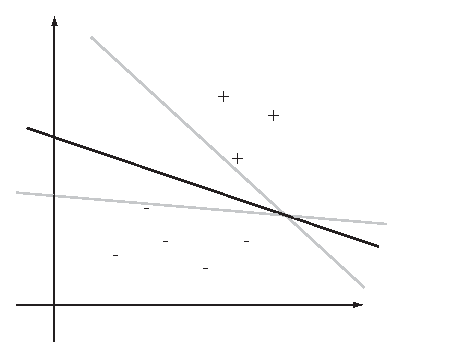
\includegraphics[height=40mm]{figures/fig06-02.eps}
\end{center}


\es



\bs{Maximum Margin Classifiers}
Characterizing the optimal decision surface.

\fdef{
A hyperplane \ul{supports a class} if it is parallel to the (linear) decision surface and all points of that class are either above or below
the supporting plane.
}

\fdef{
The distance between two supporting hyperplanes is called a \ul{margin}.
}
\es

\bs{Maximum Margin Classifiers}

We can now define decision surface optimality in terms of the margin between supporting planes:

\fdef{
A (linear) decision surface for a binary classification problem is \ul{optimal} if it is equidistant to two
supporting hyperplanes and maximizes the margin between the two supporting
hyperplanes.
}

\begin{center}
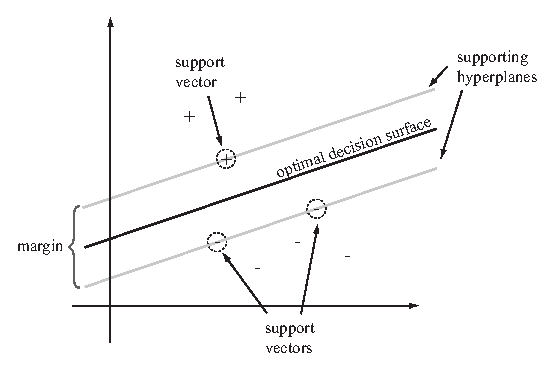
\includegraphics[height=45mm]{figures/fig06-03.eps}
\end{center}

\es

\bs{Optimality implies Optimization}
The fact that we are searching for a decision surface with an optimality  criterion such as
the `maximum margin' implies an optimization problem.

Optimization problems are problems in which we want to select the best 
solution from a number of possible or feasible solutions.
The feasible solutions are ranked by an objective function.

We define optimization problems formally,

\begin{gather*}
\min_{\ol{x}} \phi(\ol{x}), \\
\intertext{such that,}
\label{eq:opt-problem-constraints}
h_i(\ol{x}) \ge c_i,
\end{gather*}
with $i = 1,\ldots,l$ and for all $\ol{x}\in \Rnspace{n}$.  

Here, the function $\phi\co \Rnspace{n} \rightarrow \Real$ is the \ul{objective function} and
each function $h_i\co \Rnspace{n} \rightarrow \mathbb{R}$ is called a \ul{constraint} with
\ul{bound} $c_i$.

\es


\bs{Optimality implies Optimization}
Any point $\ol{x}^*$ such that $h_i(\ol{x}^*) \ge c_i$ for all $i$ is called a \ul{feasible solution}.
In addition we call $\ol{x}^*$ an \ul{optimal solution} if
\begin{equation*}
\phi(\ol{x}^*) = \min_{\ol{x}} \phi(\ol{x}), 
\end{equation*}
or
\begin{equation*}
\phi(\ol{x}^*) \le \phi(\ol{q}),
\end{equation*}
for all $\ol{q}\in \Rnspace{n}$ and $h_i(\ol{q}) \ge c_i$ for all $i$.

$\Rightarrow$ That is the optimization operator $\min$ finds the smallest feasible solution.
\es

\bs{Optimality implies Optimization}
We have defined optimization only in terms of minimization.

However, we can turn any maximization problem into a minimization problem with one of the following identities,
\begin{align*}
\max \phi(\ol{x}) &= \min -\phi(\ol{x}),\\ 
 \max \phi(\ol{x}) &= \min \frac{1}{\phi(\ol{x})}.
 \end{align*}

With the second identity we have to be careful that ${1}/{\phi(\ol{x})}$ is well defined for
all $\ol{x}$.
\es


\bs{Convex Optimization}
A convex optimization problem has a convex objective function and linear constraints. 

Convex optimization 
problems are particularly well behaved:
\begin{itemize}
\item the objective function has a global minimum,
\item the function surface is smooth in that we
can connect any two points on the function surface with a linear function without
crossing the function surface itself.
\end{itemize}

\begin{minipage}{2in}
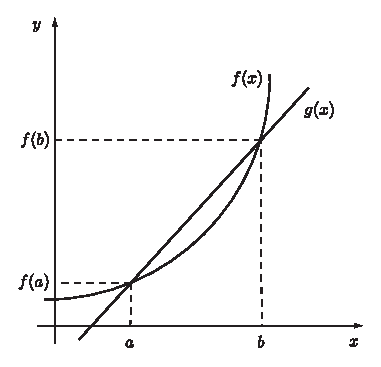
\includegraphics[height=45mm]{figures/fig06-01.eps}
\end{minipage}
\begin{minipage}{2in}
Maximizing the margin is a convex optimization problem!
\end{minipage}

\es

\bs{Projections}
\fdef{Let $\ol{a}$ and $\ol{b}$ be vectors in $\Rnspace{n}$ that form an angle $\gamma$
between them, then we say that $p_a$ is the \ul{projection} of $\ol{a}$ in the
direction of $\ol{b}$, such that,
\begin{equation*}
p_a = \abs{\ol{a}}\cos \gamma = \frac{\ol{a}\bullet\ol{b}}{\abs{b}}.
\end{equation*}
}

\vspace{.5in}
\begin{center}
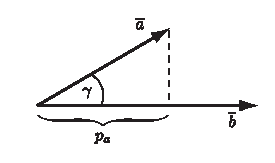
\includegraphics[height=20mm]{figures/fig06-04.eps}
\end{center}

\es


\bs{Optimizing the Margin}
Let us assume that we have a linearly separable training set,
\begin{equation*}
D = \{(\ol{x}_1,y_1),(\ol{x}_2,y_2),\ldots,(\ol{x}_l,y_l)\} \subseteq
	\Rnspace{n} \times \{+1,-1\}.
\end{equation*}
Let us also assume that we have the optimal decision surface for this training set,
\begin{equation*}
\ol{w}^*\bullet\ol{x} = b^*.
\end{equation*}
Since this decision surface is optimal, the following identities must hold,
\begin{equation*}
m^* = \phi(\ol{w}^*, b^*) = \max\phi(\ol{w},b),
\end{equation*}
where $m^*$ is the maximum margin.

\vspace{.2in}
{\bf Observation:} Our goal is to derive an expression for the objective function so that we can use it
to optimize $\ol{w}$ and $b$ and in this way obtain an optimal margin.
\es



\bs{Optimizing the Margin}
Since $\ol{w}^*\bullet\ol{x} = b^*$ is the optimal decision surface we have two supporting 
hyperplanes, say

\begin{minipage}{2in}
\begin{align*}
\ol{w}^*\bullet\ol{x} = b^* + k,\\
\ol{w}^*\bullet\ol{x} = b^* - k.
\end{align*}
with points $(\ol{x}_p, +1)$ and  $(\ol{x}_q, -1)$ in $D$ such that
\begin{align*}
\ol{w}^*\bullet\ol{x}_p = b^* + k,\\
\ol{w}^*\bullet\ol{x}_q = b^* - k.
\end{align*}
\end{minipage}
\begin{minipage}{2in}
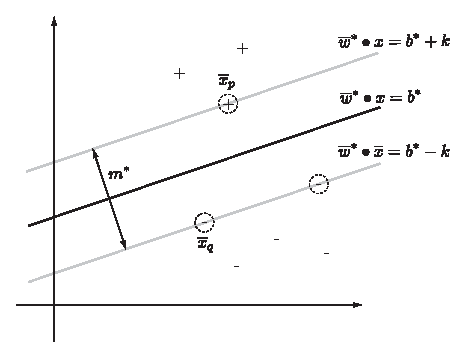
\includegraphics[height=40mm]{figures/fig06-05.eps}
\end{minipage}
\es


\bs{Optimizing the Margin}
The margin $m^*$ is the projection of $\ol{x}_p - \ol{x}_q$ onto $\ol{w}^*$.
\vspace{.2in}

\begin{minipage}{2in}
\begin{equation*}
\begin{aligned}
m^* &= \abs{\ol{x}_p - \ol{x}_q} \cos \gamma\\
	&= \frac{\ol{w}^*\bullet(\ol{x}_p - \ol{x}_q)}{\abs{\ol{w}^*}}	\\
	&=\frac{\ol{w}^*\bullet\ol{x}_p - \ol{w}^*\bullet\ol{x}_q}{\abs{\ol{w}^*}}\\
	&= \frac{(b^*+k)-(b^*-k)}{\abs{\ol{w}^*}} \\
	&=\frac{2 k}{\abs{\ol{w}^*}}.
\end{aligned}
\end{equation*}
\end{minipage}
\begin{minipage}{2in}
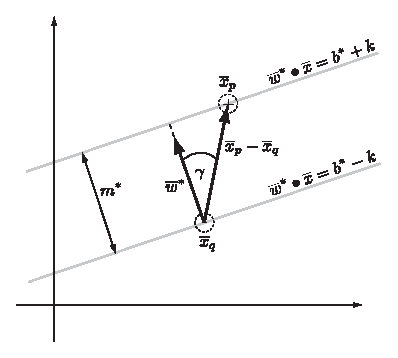
\includegraphics[height=40mm]{figures/fig06-06.eps}
\end{minipage}

\vspace{.2in}
This gives us the optimization expression, 
\begin{equation*}
\label{eq:margin-maximization1}
m^* = \max \frac{2 k}{\abs{\ol{w}}}.
\end{equation*}
\es

\bs{Optimizing the Margin}
Expressing our maximization problem as a minimization problem,
\begin{equation*}
\begin{split}
m^* &= \max \frac{2 k}{\abs{\ol{w}}} \\
	&= \min \frac{\abs{\ol{w}}}{2 k}\\
	&= \min\frac{\abs{\ol{w}}^2}{2 k}\\
	&= \min\frac{1}{2k}\ol{w}\bullet\ol{w}\\
	&= \min\frac{1}{2}\ol{w}\bullet\ol{w},
\end{split}
\end{equation*}
with $k=1$ (optimization problems are invariant under constants).

This gives us our objective function as,
\begin{equation*}
\boxed{\phi(\ol{w},b) = \frac{1}{2}\ol{w}\bullet\ol{w}.}
\end{equation*}
Note that the objective function is a convex function!
\es

\bs{Optimizing the Margin}
We can now derive the constraints for the optimization problem.  For our
optimal supporting hyperplanes the following identities hold,
\begin{align*}
\ol{w}^*\bullet\ol{x}_i&\ge b^*+k & \mbox{ for all } (\ol{x}_i,y_i)\in D\mbox{ s.t. } y_i = +1, \\
\ol{w}^*\bullet\ol{x}_i &\le b^* - k & \mbox{ for all } (\ol{x}_i,y_i)\in D\mbox{ s.t. } y_i = -1.
\end{align*}
Taking our choice of $k=1$ into account, then any feasible solution $\ol{w}\bullet\ol{x}=b$
has to fulfill the constraints,
\begin{align*}
\ol{w}\bullet\ol{x}_i&\ge 1+b & \mbox{ for all } (\ol{x}_i,y_i)\in D\mbox{ s.t. } y_i = +1, \\
\ol{w}\bullet(-\ol{x}_i) &\ge 1-b & \mbox{ for all } (\ol{x}_i,y_i)\in D\mbox{ s.t. } y_i = -1,\\
\intertext{or}
\ol{w}\bullet(y_i \ol{x}_i)&\ge 1+ y_i b & \mbox{ for all } (\ol{x}_i,y_i)\in D. 
\end{align*}
\es

\bs{Maximum Margin Classifiers}

\fframe{
{\bf Proposition:} (Maximum Margin Classifier)
Given a linearly separable training set 
\begin{equation*}
D = \{(\ol{x}_1,y_1),(\ol{x}_2,y_2),\ldots,(\ol{x}_l,y_l)\} \subseteq \Rnspace{n} \times \{+1,-1\},
\end{equation*}
we can compute a maximum margin  decision surface $\ol{w}^*\bullet\ol{x} = b^*$ with an optimization,
\begin{equation*}
\min \phi(\ol{w},b) = \min_{\ol{w},b}\frac{1}{2}\ol{w}\bullet\ol{w}
\end{equation*}
subject to the constraints,
\begin{equation*}
\ol{w}\bullet(y_i \ol{x}_i)\ge 1+ y_i b  \mbox{\hspace{.2in}\rm for all } (\ol{x}_i,y_i)\in D. 
\end{equation*}
}
\es



\end{document}
%%%%%%%%%%%%%%%%%%%%%%%%%%% end of template1.tex %%%%%%%%%%%%%%%%%%%%%%%%%%%%%%%%

